\documentclass[11pt,a4paper]{csarticle}

% --- Packages ----------------------------------------------------------------

\usepackage{amsmath,amssymb}

\usepackage{caption}
\usepackage{subcaption}
\usepackage{booktabs}
\usepackage{enumitem}
\usepackage{hyperref}

\usepackage{tcolorbox}
\tcbuselibrary{breakable,skins,listings}
\usepackage{mdframed}

\usepackage{array}
\usepackage{longtable}
\usepackage{tikz}
\usetikzlibrary{arrows.meta,positioning,automata,fit,backgrounds}

% --- Colours -----------------------------------------------------------------
\definecolor{pyblue}{HTML}{306998}
\definecolor{cppblue}{HTML}{004482}
\definecolor{shellgreen}{HTML}{2D7B2D}
\definecolor{bglight}{HTML}{F7F7F7}
\definecolor{bggray}{HTML}{EEEEEE}
\definecolor{ros2orange}{HTML}{E44D26}
\definecolor{noteblue}{HTML}{D6E4F0}
\definecolor{warnyellow}{HTML}{FFF3CD}
\definecolor{tipgreen}{HTML}{D4EDDA}

% --- Listings style ----------------------------------------------------------
\lstdefinestyle{python}{
  language=Python,
  basicstyle=\ttfamily\small,
  keywordstyle=\color{pyblue}\bfseries,
  commentstyle=\color{gray!70}\itshape,
  stringstyle=\color{orange!80!black},
  showstringspaces=false,
  numbers=left,
  numberstyle=\tiny\color{gray},
  stepnumber=1,
  numbersep=8pt,
  backgroundcolor=\color{bglight},
  frame=single,
  rulecolor=\color{pyblue!40},
  breaklines=true,
  breakatwhitespace=false,
  tabsize=4,
  captionpos=b,
  morekeywords={self,True,False,None,import,from,as,def,class,return,if,else,
                elif,for,while,with,yield,lambda,pass,raise,try,except,finally},
}

\lstdefinestyle{cpp}{
  language=C++,
  basicstyle=\ttfamily\small,
  keywordstyle=\color{cppblue}\bfseries,
  commentstyle=\color{gray!70}\itshape,
  stringstyle=\color{orange!80!black},
  showstringspaces=false,
  numbers=left,
  numberstyle=\tiny\color{gray},
  stepnumber=1,
  numbersep=8pt,
  backgroundcolor=\color{bglight},
  frame=single,
  rulecolor=\color{cppblue!40},
  breaklines=true,
  breakatwhitespace=false,
  tabsize=2,
  captionpos=b,
  morecomment=[l]{//},
  morecomment=[s]{/*}{*/},
}

\lstdefinestyle{bash}{
  language=bash,
  basicstyle=\ttfamily\small,
  keywordstyle=\color{shellgreen}\bfseries,
  commentstyle=\color{gray!70}\itshape,
  stringstyle=\color{orange!80!black},
  showstringspaces=false,
  numbers=none,
  backgroundcolor=\color{black!90},
  basicstyle=\ttfamily\small\color{white},
  frame=single,
  rulecolor=\color{black},
  breaklines=true,
  tabsize=2,
  captionpos=b,
}

\lstdefinestyle{xml}{
  language=XML,
  basicstyle=\ttfamily\small,
  keywordstyle=\color{purple!70!black}\bfseries,
  commentstyle=\color{gray!70}\itshape,
  stringstyle=\color{orange!80!black},
  showstringspaces=false,
  numbers=left,
  numberstyle=\tiny\color{gray},
  stepnumber=1,
  numbersep=8pt,
  backgroundcolor=\color{bglight},
  frame=single,
  rulecolor=\color{purple!40},
  breaklines=true,
  tabsize=2,
  captionpos=b,
}

% --- tcolorbox environments ---------------------------------------------------
\newtcolorbox{notebox}{
  breakable,
  colback=noteblue,
  colframe=blue!60!black,
  fonttitle=\bfseries,
  title={Note},
  left=4pt, right=4pt, top=4pt, bottom=4pt,
}

\newtcolorbox{warnbox}{
  breakable,
  colback=warnyellow,
  colframe=orange!80!black,
  fonttitle=\bfseries,
  title={Warning},
  left=4pt, right=4pt, top=4pt, bottom=4pt,
}

\newtcolorbox{tipbox}{
  breakable,
  colback=tipgreen,
  colframe=green!50!black,
  fonttitle=\bfseries,
  title={Tip},
  left=4pt, right=4pt, top=4pt, bottom=4pt,
}


% --- Misc helpers -------------------------------------------------------------
\newcommand{\ros}{\texttt{ROS~2}\xspace}
%\newcommand{\code}[1]{\texttt{#1}}
\newcommand{\pkg}[1]{\textbf{\texttt{#1}}}

% -----------------------------------------------------------------------------
\begin{document}

% --- Title page --------------------------------------------------------------
\title{ROS~2 Lifecycle Nodes}
\subtitle{A Complete Tutorial with Python \& C++ Examples\\
	Covers: Humble / Iron / Jazzy distributions}
\author{Claude}
\version{1.0}
\date{\today}
\abstract{This document is a self-contained tutorial on ROS~2 \emph{Lifecycle Nodes}.
    It includes full code examples in both Python and C++, build-system files,
    command-line usage, and a hands-on walkthrough.  Appendix~\ref{app:install}
    covers installation of ROS~2 and workspace preparation on Ubuntu Linux.}

\maketitle
\printabstract
\tableofcontents

% -----------------------------------------------------------------------------
\section{Introduction}
\label{sec:intro}
% -----------------------------------------------------------------------------

\subsection{What is a Lifecycle Node?}

In standard ROS~2, a node starts executing immediately upon creation, and the
only way to stop it is to kill the process.  This makes it difficult to
coordinate the startup and shutdown of complex multi-node systems.

\textbf{Lifecycle Nodes} (also called \emph{managed nodes}) address this by
giving each node a well-defined state machine.  A lifecycle node does not
begin meaningful work until it is explicitly told to do so by an external
manager or by user commands.  The operator can also pause, reconfigure, and
cleanly shut down the node at run-time without restarting the whole system.

Lifecycle nodes are standardised in
\href{https://design.ros2.org/articles/node_lifecycle.html}{REP~2006} and
implemented in the \pkg{rclcpp\_lifecycle} (C++) and
\pkg{rclpy} (Python, via \xcode{LifecycleNode}) packages.

\subsection{Why Use Lifecycle Nodes?}

\begin{itemize}[noitemsep]
  \item \textbf{Deterministic start-up}: ensure all dependencies are ready
        before a node becomes active.
  \item \textbf{Safe configuration}: allocate hardware resources only when
        needed; release them cleanly on shutdown.
  \item \textbf{Fault isolation}: deactivate a misbehaving node without
        restarting the entire robot pipeline.
  \item \textbf{System orchestration}: a \emph{lifecycle manager}
        (e.g.\ from \pkg{nav2\_lifecycle\_manager}) can supervise multiple
        nodes as a unit.
  \item \textbf{Better testing}: each state transition can be unit-tested
        independently.
\end{itemize}

\subsection{Scope of this Tutorial}

\begin{enumerate}[noitemsep]
  \item The lifecycle state machine in detail.
  \item Writing lifecycle nodes in \textbf{Python} and \textbf{C++}.
  \item Building with \xcode{colcon} and \xcode{CMake}/\xcode{setuptools}.
  \item Triggering transitions from the command line and programmatically.
  \item Monitoring state via services and topics.
  \item Implementing a simple lifecycle manager.
  \item Best practices and common pitfalls.
  \item Appendix: installing ROS~2 and setting up a workspace on Ubuntu.
\end{enumerate}

% -----------------------------------------------------------------------------
\section{The Lifecycle State Machine}
\label{sec:statemachine}
% -----------------------------------------------------------------------------

\subsection{Primary States}

A lifecycle node always resides in one of the following \emph{primary states}:

\begin{center}
\begin{tabular}{lp{9cm}}
  \toprule
  \textbf{State} & \textbf{Description} \\
  \midrule
  \texttt{Unconfigured} & Node has been created but not yet configured.
                           No publishers, subscribers, or timers are active. \\
  \texttt{Inactive}     & Node has been configured (resources allocated) but
                           is not processing data. \\
  \texttt{Active}       & Node is fully operational and processing data. \\
  \texttt{Finalized}    & Node has been shut down and cannot be restarted. \\
  \bottomrule
\end{tabular}
\end{center}

\subsection{Transition States}

Between primary states the node briefly enters a \emph{transition state}
while executing callback logic.  If the callback succeeds the node moves to
the target primary state; if it fails the node moves to an error state
instead.

\begin{center}
\begin{tabular}{llll}
  \toprule
  \textbf{Transition} & \textbf{From} & \textbf{To (success)} & \textbf{To (failure)} \\
  \midrule
  \texttt{configure}   & Unconfigured & Inactive     & Unconfigured \\
  \texttt{activate}    & Inactive     & Active       & Inactive \\
  \texttt{deactivate}  & Active       & Inactive     & Active \\
  \texttt{cleanup}     & Inactive     & Unconfigured & Inactive \\
  \texttt{shutdown}    & Any primary  & Finalized    & Finalized \\
  \texttt{error}       & Any          & Unconfigured & Finalized \\
  \bottomrule
\end{tabular}
\end{center}

\subsection{Transition Callbacks}

Each transition maps to a callback that you override in your node class:

\begin{center}
\begin{tabular}{ll}
  \toprule
  \textbf{Callback} & \textbf{Triggered by} \\
  \midrule
  \xcode{on\_configure}   & \texttt{configure} transition \\
  \xcode{on\_activate}    & \texttt{activate} transition \\
  \xcode{on\_deactivate}  & \texttt{deactivate} transition \\
  \xcode{on\_cleanup}     & \texttt{cleanup} transition \\
  \xcode{on\_shutdown}    & \texttt{shutdown} transition \\
  \xcode{on\_error}       & Error recovery \\
  \bottomrule
\end{tabular}
\end{center}

All callbacks must return a \emph{transition result}:

\begin{itemize}[noitemsep]
  \item \textbf{Python}: return \xcode{TransitionCallbackReturn.SUCCESS},
        \xcode{.FAILURE}, or \xcode{.ERROR}.
  \item \textbf{C++}: return \xcode{CallbackReturn::SUCCESS},
        \xcode{CallbackReturn::FAILURE}, or \xcode{CallbackReturn::ERROR}.
\end{itemize}

\subsection{Full State-Machine Diagram}

\begin{center}
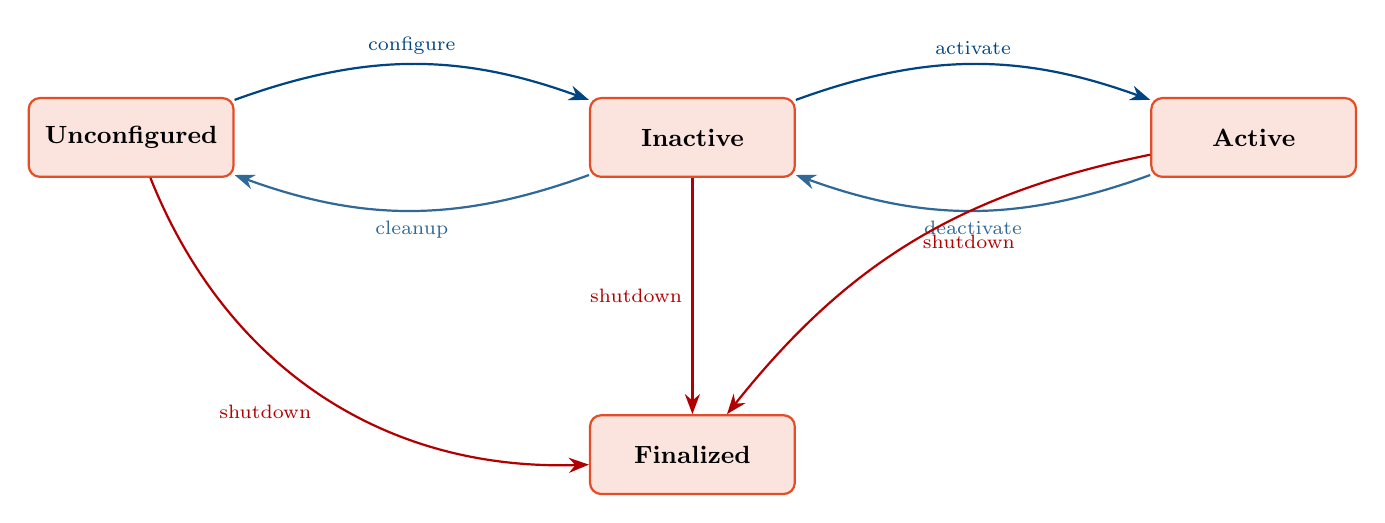
\begin{tikzpicture}[
  node distance=2.8cm and 4cm,
  pstate/.style={draw,rectangle,rounded corners=4pt,minimum width=2.6cm,minimum height=1cm,
                 thick,fill=ros2orange!15,draw=ros2orange,font=\small\bfseries},
  tstate/.style={draw,rectangle,minimum width=2.4cm,minimum height=0.7cm,
                 thick,fill=gray!15,draw=gray!60,font=\scriptsize\itshape},
  every edge/.style={draw,thick,-{Stealth[scale=1.1]}},
]
  % Primary states
  \node[pstate] (unc) {Unconfigured};
  \node[pstate,right=4.5cm of unc] (ina) {Inactive};
  \node[pstate,right=4.5cm of ina] (act) {Active};
  \node[pstate,below=3cm of ina]   (fin) {Finalized};

  % Arrows
  \draw[color=cppblue,bend left=20]  (unc) edge node[above,font=\scriptsize,color=cppblue]{configure}  (ina);
  \draw[color=pyblue,bend left=20]   (ina) edge node[below,font=\scriptsize,color=pyblue]{cleanup}     (unc);
  \draw[color=cppblue,bend left=20]  (ina) edge node[above,font=\scriptsize,color=cppblue]{activate}   (act);
  \draw[color=pyblue,bend left=20]   (act) edge node[below,font=\scriptsize,color=pyblue]{deactivate}  (ina);
  \draw[color=red!70!black]          (ina) edge node[left, font=\scriptsize]{shutdown}  (fin);
  \draw[color=red!70!black,bend right=20] (act) edge node[right,font=\scriptsize]{shutdown} (fin);
  \draw[color=red!70!black,bend right=35] (unc) edge node[below left,font=\scriptsize]{shutdown} (fin);
\end{tikzpicture}
\end{center}

% -----------------------------------------------------------------------------
\section{Lifecycle Nodes in Python}
\label{sec:python}
% -----------------------------------------------------------------------------

\subsection{Package Structure}

\begin{lstlisting}[style=bash,caption={Python package layout}]
my_lifecycle_py/
  my_lifecycle_py/
    __init__.py
    lifecycle_talker.py      # publisher lifecycle node
    lifecycle_listener.py    # subscriber lifecycle node
    lifecycle_manager.py     # simple manager node
  resource/
    my_lifecycle_py
  package.xml
  setup.cfg
  setup.py
\end{lstlisting}

\subsection{package.xml}

\begin{lstlisting}[style=xml,caption={package.xml for the Python package}]
<?xml version="1.0"?>
<?xml-model href="http://download.ros.org/schema/package_format3.xsd"
            schematypens="http://www.w3.org/2001/XMLSchema"?>
<package format="3">
  <name>my_lifecycle_py</name>
  <version>0.1.0</version>
  <description>ROS 2 lifecycle node examples in Python</description>
  <maintainer email="dev@example.com">Developer</maintainer>
  <license>Apache-2.0</license>

  <exec_depend>rclpy</exec_depend>
  <exec_depend>lifecycle_msgs</exec_depend>
  <exec_depend>std_msgs</exec_depend>

  <test_depend>ament_copyright</test_depend>
  <test_depend>ament_flake8</test_depend>
  <test_depend>ament_pep257</test_depend>

  <export>
    <build_type>ament_python</build_type>
  </export>
</package>
\end{lstlisting}

\subsection{setup.py}

\begin{lstlisting}[style=python,caption={setup.py}]
from setuptools import setup

package_name = 'my_lifecycle_py'

setup(
    name=package_name,
    version='0.1.0',
    packages=[package_name],
    data_files=[
        ('share/ament_index/resource_index/packages',
         ['resource/' + package_name]),
        ('share/' + package_name, ['package.xml']),
    ],
    install_requires=['setuptools'],
    zip_safe=True,
    maintainer='Developer',
    maintainer_email='dev@example.com',
    description='ROS 2 lifecycle node examples in Python',
    license='Apache-2.0',
    entry_points={
        'console_scripts': [
            'lifecycle_talker   = my_lifecycle_py.lifecycle_talker:main',
            'lifecycle_listener = my_lifecycle_py.lifecycle_listener:main',
            'lifecycle_manager  = my_lifecycle_py.lifecycle_manager:main',
        ],
    },
)
\end{lstlisting}

\subsection{Python -- Lifecycle Talker (Publisher Node)}
\label{sec:py-talker}

The following example implements a lifecycle node that publishes a
\xcode{std\_msgs/String} message only while in the \emph{Active} state.
It demonstrates the four main transition callbacks.

\begin{lstlisting}[style=python,caption={lifecycle\_talker.py -- full example}]
# Copyright 2024 Developer
# SPDX-License-Identifier: Apache-2.0
"""Lifecycle talker: publishes only while Active."""

import rclpy
from rclpy.lifecycle import LifecycleNode
from rclpy.lifecycle import TransitionCallbackReturn
from rclpy.lifecycle import State
from rclpy.timer import Timer
from std_msgs.msg import String


class LifecycleTalker(LifecycleNode):
    """A lifecycle node that publishes 'Hello' messages."""

    def __init__(self, node_name: str, **kwargs) -> None:
        """Initialise without creating ROS entities yet."""
        super().__init__(node_name, **kwargs)
        self._pub = None
        self._timer: Timer | None = None
        self._count: int = 0
        self.get_logger().info('LifecycleTalker created (Unconfigured)')

    # -- Transition callbacks ----------------------------------------------

    def on_configure(self, state: State) -> TransitionCallbackReturn:
        """Allocate resources: create publisher.

        Called by the 'configure' transition.
        Returning SUCCESS moves the node to Inactive.
        """
        self.get_logger().info(
            f'Configuring from state: {state.label}')

        # Create publisher -- it exists but is NOT active yet
        self._pub = self.create_lifecycle_publisher(
            String, 'lifecycle_chatter', 10)

        self._count = 0
        self.get_logger().info('Publisher created.')
        return TransitionCallbackReturn.SUCCESS

    def on_activate(self, state: State) -> TransitionCallbackReturn:
        """Start publishing: create a timer that fires every second.

        Called by the 'activate' transition.
        Returning SUCCESS moves the node to Active.
        """
        self.get_logger().info(
            f'Activating from state: {state.label}')

        # Timer is created here so it fires only in Active state
        self._timer = self.create_timer(1.0, self._timer_callback)

        # IMPORTANT: call super().on_activate() to activate the publisher
        return super().on_activate(state)

    def on_deactivate(self, state: State) -> TransitionCallbackReturn:
        """Pause publishing: destroy the timer.

        Called by the 'deactivate' transition.
        Returning SUCCESS moves the node to Inactive.
        """
        self.get_logger().info(
            f'Deactivating from state: {state.label}')

        if self._timer:
            self._timer.destroy()
            self._timer = None

        # Call super to deactivate the publisher
        return super().on_deactivate(state)

    def on_cleanup(self, state: State) -> TransitionCallbackReturn:
        """Release all resources.

        Called by the 'cleanup' transition.
        Returning SUCCESS moves the node back to Unconfigured.
        """
        self.get_logger().info(
            f'Cleaning up from state: {state.label}')

        if self._timer:
            self._timer.destroy()
            self._timer = None

        if self._pub:
            self.destroy_publisher(self._pub)
            self._pub = None

        self._count = 0
        self.get_logger().info('Resources released.')
        return TransitionCallbackReturn.SUCCESS

    def on_shutdown(self, state: State) -> TransitionCallbackReturn:
        """Graceful shutdown -- called from any primary state."""
        self.get_logger().info(
            f'Shutting down from state: {state.label}')

        # Re-use cleanup logic
        if self._timer:
            self._timer.destroy()
            self._timer = None
        if self._pub:
            self.destroy_publisher(self._pub)
            self._pub = None

        return TransitionCallbackReturn.SUCCESS

    def on_error(self, state: State) -> TransitionCallbackReturn:
        """Error recovery handler."""
        self.get_logger().error(
            f'Error in state: {state.label}. Attempting recovery.')
        # Attempt to clean up; returning FAILURE sends to Finalized
        return TransitionCallbackReturn.SUCCESS

    # -- Internal ---------------------------------------------------------

    def _timer_callback(self) -> None:
        """Publish a message. Only called while Active."""
        if self._pub and self._pub.is_activated:
            msg = String()
            msg.data = f'Hello, lifecycle world! count={self._count}'
            self._pub.publish(msg)
            self.get_logger().info(f'Published: "{msg.data}"')
            self._count += 1


def main(args=None):
    rclpy.init(args=args)
    node = LifecycleTalker('lifecycle_talker')
    executor = rclpy.executors.SingleThreadedExecutor()
    executor.add_node(node)
    try:
        executor.spin()
    except KeyboardInterrupt:
        pass
    finally:
        node.destroy_node()
        rclpy.shutdown()


if __name__ == '__main__':
    main()
\end{lstlisting}

\begin{notebox}
  \textbf{Key point}: use \xcode{create\_lifecycle\_publisher()} instead of
  \xcode{create\_publisher()}.  A lifecycle publisher is automatically
  \emph{activated} and \emph{deactivated} with the node, preventing messages
  from being published in the wrong state.  Always call
  \xcode{super().on\_activate(state)} and \xcode{super().on\_deactivate(state)}
  to trigger this behaviour.
\end{notebox}

\subsection{Python -- Lifecycle Listener (Subscriber Node)}

\begin{lstlisting}[style=python,caption={lifecycle\_listener.py}]
# Copyright 2024 Developer
# SPDX-License-Identifier: Apache-2.0
"""Lifecycle listener: receives messages only while Active."""

import rclpy
from rclpy.lifecycle import LifecycleNode
from rclpy.lifecycle import TransitionCallbackReturn
from rclpy.lifecycle import State
from std_msgs.msg import String


class LifecycleListener(LifecycleNode):
    """A lifecycle node that subscribes to the chatter topic."""

    def __init__(self, node_name: str, **kwargs) -> None:
        super().__init__(node_name, **kwargs)
        self._sub = None
        self.get_logger().info('LifecycleListener created (Unconfigured)')

    def on_configure(self, state: State) -> TransitionCallbackReturn:
        self.get_logger().info('Configuring listener...')
        # Subscription is created here; messages are queued but the
        # callback fires only when the node is Active.
        self._sub = self.create_subscription(
            String,
            'lifecycle_chatter',
            self._chatter_callback,
            10,
        )
        return TransitionCallbackReturn.SUCCESS

    def on_activate(self, state: State) -> TransitionCallbackReturn:
        self.get_logger().info('Activating listener...')
        return super().on_activate(state)

    def on_deactivate(self, state: State) -> TransitionCallbackReturn:
        self.get_logger().info('Deactivating listener...')
        return super().on_deactivate(state)

    def on_cleanup(self, state: State) -> TransitionCallbackReturn:
        self.get_logger().info('Cleaning up listener...')
        if self._sub:
            self.destroy_subscription(self._sub)
            self._sub = None
        return TransitionCallbackReturn.SUCCESS

    def on_shutdown(self, state: State) -> TransitionCallbackReturn:
        self.get_logger().info('Shutting down listener...')
        if self._sub:
            self.destroy_subscription(self._sub)
            self._sub = None
        return TransitionCallbackReturn.SUCCESS

    def _chatter_callback(self, msg: String) -> None:
        self.get_logger().info(f'Received: "{msg.data}"')


def main(args=None):
    rclpy.init(args=args)
    node = LifecycleListener('lifecycle_listener')
    executor = rclpy.executors.SingleThreadedExecutor()
    executor.add_node(node)
    try:
        executor.spin()
    except KeyboardInterrupt:
        pass
    finally:
        node.destroy_node()
        rclpy.shutdown()


if __name__ == '__main__':
    main()
\end{lstlisting}

\subsection{Python -- Programmatic Lifecycle Manager}
\label{sec:py-manager}

The following node drives another lifecycle node through its states
programmatically by calling lifecycle change-state services.

\begin{lstlisting}[style=python,caption={lifecycle\_manager.py}]
# Copyright 2024 Developer
# SPDX-License-Identifier: Apache-2.0
"""Simple lifecycle manager that drives another node through its states."""

import time
import rclpy
from rclpy.node import Node
from lifecycle_msgs.srv import ChangeState, GetState
from lifecycle_msgs.msg import Transition


TRANSITIONS = {
    'configure':  Transition.TRANSITION_CONFIGURE,
    'activate':   Transition.TRANSITION_ACTIVATE,
    'deactivate': Transition.TRANSITION_DEACTIVATE,
    'cleanup':    Transition.TRANSITION_CLEANUP,
    'shutdown':   Transition.TRANSITION_UNCONFIGURED_SHUTDOWN,
}


class LifecycleManager(Node):
    """Drives a target lifecycle node through a predefined sequence."""

    def __init__(self, target_node: str = 'lifecycle_talker') -> None:
        super().__init__('lifecycle_manager')
        self._target = target_node

        # Create service clients
        self._change_state = self.create_client(
            ChangeState,
            f'/{target_node}/change_state',
        )
        self._get_state = self.create_client(
            GetState,
            f'/{target_node}/get_state',
        )
        self.get_logger().info(
            f'LifecycleManager ready to manage: {target_node}')

    # -- Public API --------------------------------------------------------

    def get_state(self) -> str | None:
        """Return the current primary state label of the managed node."""
        if not self._get_state.wait_for_service(timeout_sec=5.0):
            self.get_logger().error('get_state service not available')
            return None
        future = self._get_state.call_async(GetState.Request())
        rclpy.spin_until_future_complete(self, future, timeout_sec=5.0)
        if future.result():
            return future.result().current_state.label
        return None

    def change_state(self, transition_name: str) -> bool:
        """Trigger a named transition. Returns True on success."""
        if transition_name not in TRANSITIONS:
            self.get_logger().error(
                f'Unknown transition: {transition_name}')
            return False

        if not self._change_state.wait_for_service(timeout_sec=5.0):
            self.get_logger().error('change_state service not available')
            return False

        req = ChangeState.Request()
        req.transition.id = TRANSITIONS[transition_name]
        req.transition.label = transition_name

        future = self._change_state.call_async(req)
        rclpy.spin_until_future_complete(self, future, timeout_sec=10.0)

        if future.result() and future.result().success:
            state = self.get_state()
            self.get_logger().info(
                f'Transition "{transition_name}" succeeded. '
                f'New state: {state}')
            return True
        else:
            self.get_logger().error(
                f'Transition "{transition_name}" FAILED.')
            return False

    def run_demo_sequence(self) -> None:
        """Run configure -> activate -> (wait) -> deactivate -> cleanup."""
        steps = [
            ('configure',  2.0),
            ('activate',   5.0),
            ('deactivate', 1.0),
            ('cleanup',    1.0),
        ]
        for transition, wait in steps:
            if not self.change_state(transition):
                self.get_logger().error(
                    f'Aborting sequence at: {transition}')
                return
            time.sleep(wait)

        self.get_logger().info('Demo sequence complete.')


def main(args=None):
    rclpy.init(args=args)
    manager = LifecycleManager(target_node='lifecycle_talker')

    # Wait briefly for the talker to come up
    time.sleep(2.0)
    manager.run_demo_sequence()

    manager.destroy_node()
    rclpy.shutdown()


if __name__ == '__main__':
    main()
\end{lstlisting}

% -----------------------------------------------------------------------------
\section{Lifecycle Nodes in C++}
\label{sec:cpp}
% -----------------------------------------------------------------------------

\subsection{Package Structure}

\begin{lstlisting}[style=bash,caption={C++ package layout}]
my_lifecycle_cpp/
  include/
    my_lifecycle_cpp/
      lifecycle_talker.hpp
      lifecycle_listener.hpp
      lifecycle_manager.hpp
  src/
    lifecycle_talker.cpp
    lifecycle_listener.cpp
    lifecycle_manager.cpp
  package.xml
  CMakeLists.txt
\end{lstlisting}

\subsection{package.xml}

\begin{lstlisting}[style=xml,caption={package.xml for the C++ package}]
<?xml version="1.0"?>
<package format="3">
  <name>my_lifecycle_cpp</name>
  <version>0.1.0</version>
  <description>ROS 2 lifecycle node examples in C++</description>
  <maintainer email="dev@example.com">Developer</maintainer>
  <license>Apache-2.0</license>

  <buildtool_depend>ament_cmake</buildtool_depend>

  <depend>rclcpp</depend>
  <depend>rclcpp_lifecycle</depend>
  <depend>lifecycle_msgs</depend>
  <depend>std_msgs</depend>

  <test_depend>ament_lint_auto</test_depend>
  <test_depend>ament_lint_common</test_depend>

  <export>
    <build_type>ament_cmake</build_type>
  </export>
</package>
\end{lstlisting}

\subsection{CMakeLists.txt}

\begin{lstlisting}[style=bash,caption={CMakeLists.txt}]
cmake_minimum_required(VERSION 3.14)
project(my_lifecycle_cpp)

# C++17 required for std::optional, structured bindings, etc.
if(NOT CMAKE_CXX_STANDARD)
  set(CMAKE_CXX_STANDARD 17)
endif()
if(CMAKE_COMPILER_IS_GNUCXX OR CMAKE_CXX_COMPILER_ID MATCHES "Clang")
  add_compile_options(-Wall -Wextra -Wpedantic)
endif()

# Find dependencies
find_package(ament_cmake REQUIRED)
find_package(rclcpp REQUIRED)
find_package(rclcpp_lifecycle REQUIRED)
find_package(lifecycle_msgs REQUIRED)
find_package(std_msgs REQUIRED)

set(DEPS
  rclcpp rclcpp_lifecycle lifecycle_msgs std_msgs)

# -- Lifecycle Talker ----------------------------------------------------------
add_executable(lifecycle_talker src/lifecycle_talker.cpp)
ament_target_dependencies(lifecycle_talker ${DEPS})
target_include_directories(lifecycle_talker PUBLIC
  $<BUILD_INTERFACE:${CMAKE_CURRENT_SOURCE_DIR}/include>)

# -- Lifecycle Listener --------------------------------------------------------
add_executable(lifecycle_listener src/lifecycle_listener.cpp)
ament_target_dependencies(lifecycle_listener ${DEPS})
target_include_directories(lifecycle_listener PUBLIC
  $<BUILD_INTERFACE:${CMAKE_CURRENT_SOURCE_DIR}/include>)

# -- Lifecycle Manager ---------------------------------------------------------
add_executable(lifecycle_manager src/lifecycle_manager.cpp)
ament_target_dependencies(lifecycle_manager ${DEPS})
target_include_directories(lifecycle_manager PUBLIC
  $<BUILD_INTERFACE:${CMAKE_CURRENT_SOURCE_DIR}/include>)

# Install
install(TARGETS
  lifecycle_talker lifecycle_listener lifecycle_manager
  DESTINATION lib/${PROJECT_NAME})

if(BUILD_TESTING)
  find_package(ament_lint_auto REQUIRED)
  ament_lint_auto_find_test_dependencies()
endif()

ament_package()
\end{lstlisting}

\subsection{C++ -- Lifecycle Talker Header}

\begin{lstlisting}[style=cpp,caption={include/my\_lifecycle\_cpp/lifecycle\_talker.hpp}]
// Copyright 2024 Developer
// SPDX-License-Identifier: Apache-2.0
#ifndef MY_LIFECYCLE_CPP__LIFECYCLE_TALKER_HPP_
#define MY_LIFECYCLE_CPP__LIFECYCLE_TALKER_HPP_

#include <memory>
#include <string>

#include "rclcpp/rclcpp.hpp"
#include "rclcpp_lifecycle/lifecycle_node.hpp"
#include "rclcpp_lifecycle/lifecycle_publisher.hpp"
#include "std_msgs/msg/string.hpp"

namespace my_lifecycle_cpp
{

using CallbackReturn =
  rclcpp_lifecycle::node_interfaces::LifecycleNodeInterface::CallbackReturn;

/**
 * @brief Lifecycle talker node.
 *
 * Publishes std_msgs::msg::String messages at 1 Hz only while Active.
 */
class LifecycleTalker : public rclcpp_lifecycle::LifecycleNode
{
public:
  /**
   * @brief Construct the talker.
   * @param options  Node options forwarded to LifecycleNode.
   */
  explicit LifecycleTalker(
    const rclcpp::NodeOptions & options = rclcpp::NodeOptions());

  ~LifecycleTalker() override = default;

  // -- Transition callbacks -------------------------------------------------
  CallbackReturn on_configure(const rclcpp_lifecycle::State & state) override;
  CallbackReturn on_activate  (const rclcpp_lifecycle::State & state) override;
  CallbackReturn on_deactivate(const rclcpp_lifecycle::State & state) override;
  CallbackReturn on_cleanup   (const rclcpp_lifecycle::State & state) override;
  CallbackReturn on_shutdown  (const rclcpp_lifecycle::State & state) override;

private:
  void timer_callback();

  rclcpp_lifecycle::LifecyclePublisher<std_msgs::msg::String>::SharedPtr pub_;
  rclcpp::TimerBase::SharedPtr timer_;
  size_t count_{0};
};

}  // namespace my_lifecycle_cpp
#endif  // MY_LIFECYCLE_CPP__LIFECYCLE_TALKER_HPP_
\end{lstlisting}

\subsection{C++ -- Lifecycle Talker Implementation}

\begin{lstlisting}[style=cpp,caption={src/lifecycle\_talker.cpp}]
// Copyright 2024 Developer
// SPDX-License-Identifier: Apache-2.0
#include "my_lifecycle_cpp/lifecycle_talker.hpp"

#include <chrono>
#include <memory>
#include <string>

using namespace std::chrono_literals;

namespace my_lifecycle_cpp
{

LifecycleTalker::LifecycleTalker(const rclcpp::NodeOptions & options)
: rclcpp_lifecycle::LifecycleNode("lifecycle_talker", options)
{
  RCLCPP_INFO(get_logger(), "LifecycleTalker created (Unconfigured)");
}

// -- on_configure -------------------------------------------------------------
CallbackReturn
LifecycleTalker::on_configure(const rclcpp_lifecycle::State & state)
{
  RCLCPP_INFO(get_logger(),
    "Configuring from state: %s", state.label().c_str());

  // Create a lifecycle publisher.
  // It is inactive until on_activate() is called.
  pub_ = create_lifecycle_publisher<std_msgs::msg::String>(
    "lifecycle_chatter", 10);

  count_ = 0;
  RCLCPP_INFO(get_logger(), "Publisher created.");
  return CallbackReturn::SUCCESS;
}

// -- on_activate --------------------------------------------------------------
CallbackReturn
LifecycleTalker::on_activate(const rclcpp_lifecycle::State & state)
{
  RCLCPP_INFO(get_logger(),
    "Activating from state: %s", state.label().c_str());

  // Create the timer that triggers publishing
  timer_ = create_wall_timer(
    1s, std::bind(&LifecycleTalker::timer_callback, this));

  // IMPORTANT: call the parent implementation to activate the publisher
  LifecycleNode::on_activate(state);
  return CallbackReturn::SUCCESS;
}

// -- on_deactivate -------------------------------------------------------------
CallbackReturn
LifecycleTalker::on_deactivate(const rclcpp_lifecycle::State & state)
{
  RCLCPP_INFO(get_logger(),
    "Deactivating from state: %s", state.label().c_str());

  // Destroy the timer to stop publishing
  timer_.reset();

  // Deactivate the publisher through the parent
  LifecycleNode::on_deactivate(state);
  return CallbackReturn::SUCCESS;
}

// -- on_cleanup ---------------------------------------------------------------
CallbackReturn
LifecycleTalker::on_cleanup(const rclcpp_lifecycle::State & state)
{
  RCLCPP_INFO(get_logger(),
    "Cleaning up from state: %s", state.label().c_str());

  timer_.reset();
  pub_.reset();
  count_ = 0;
  RCLCPP_INFO(get_logger(), "Resources released.");
  return CallbackReturn::SUCCESS;
}

// -- on_shutdown --------------------------------------------------------------
CallbackReturn
LifecycleTalker::on_shutdown(const rclcpp_lifecycle::State & state)
{
  RCLCPP_INFO(get_logger(),
    "Shutting down from state: %s", state.label().c_str());

  timer_.reset();
  pub_.reset();
  return CallbackReturn::SUCCESS;
}

// -- timer_callback ------------------------------------------------------------
void LifecycleTalker::timer_callback()
{
  if (!pub_ || !pub_->is_activated()) {
    return;
  }
  auto msg = std_msgs::msg::String();
  msg.data = "Hello, lifecycle world! count=" + std::to_string(count_++);
  pub_->publish(msg);
  RCLCPP_INFO(get_logger(), "Published: '%s'", msg.data.c_str());
}

}  // namespace my_lifecycle_cpp

// -- main ---------------------------------------------------------------------
int main(int argc, char ** argv)
{
  rclcpp::init(argc, argv);
  auto node = std::make_shared<my_lifecycle_cpp::LifecycleTalker>();
  rclcpp::spin(node->get_node_base_interface());
  rclcpp::shutdown();
  return 0;
}
\end{lstlisting}

\subsection{C++ -- Lifecycle Listener Header}

\begin{lstlisting}[style=cpp,caption={include/my\_lifecycle\_cpp/lifecycle\_listener.hpp}]
// Copyright 2024 Developer
// SPDX-License-Identifier: Apache-2.0
#ifndef MY_LIFECYCLE_CPP__LIFECYCLE_LISTENER_HPP_
#define MY_LIFECYCLE_CPP__LIFECYCLE_LISTENER_HPP_

#include <memory>

#include "rclcpp/rclcpp.hpp"
#include "rclcpp_lifecycle/lifecycle_node.hpp"
#include "std_msgs/msg/string.hpp"

namespace my_lifecycle_cpp
{

using CallbackReturn =
  rclcpp_lifecycle::node_interfaces::LifecycleNodeInterface::CallbackReturn;

class LifecycleListener : public rclcpp_lifecycle::LifecycleNode
{
public:
  explicit LifecycleListener(
    const rclcpp::NodeOptions & options = rclcpp::NodeOptions());

  CallbackReturn on_configure (const rclcpp_lifecycle::State &) override;
  CallbackReturn on_activate  (const rclcpp_lifecycle::State &) override;
  CallbackReturn on_deactivate(const rclcpp_lifecycle::State &) override;
  CallbackReturn on_cleanup   (const rclcpp_lifecycle::State &) override;
  CallbackReturn on_shutdown  (const rclcpp_lifecycle::State &) override;

private:
  void chatter_callback(const std_msgs::msg::String & msg);
  rclcpp::Subscription<std_msgs::msg::String>::SharedPtr sub_;
};

}  // namespace my_lifecycle_cpp
#endif  // MY_LIFECYCLE_CPP__LIFECYCLE_LISTENER_HPP_
\end{lstlisting}

\subsection{C++ -- Lifecycle Listener Implementation}

\begin{lstlisting}[style=cpp,caption={src/lifecycle\_listener.cpp}]
// Copyright 2024 Developer
// SPDX-License-Identifier: Apache-2.0
#include "my_lifecycle_cpp/lifecycle_listener.hpp"

#include <memory>
#include <functional>

namespace my_lifecycle_cpp
{

LifecycleListener::LifecycleListener(const rclcpp::NodeOptions & opts)
: rclcpp_lifecycle::LifecycleNode("lifecycle_listener", opts)
{
  RCLCPP_INFO(get_logger(), "LifecycleListener created (Unconfigured)");
}

CallbackReturn
LifecycleListener::on_configure(const rclcpp_lifecycle::State & state)
{
  RCLCPP_INFO(get_logger(), "Configuring: %s", state.label().c_str());
  sub_ = create_subscription<std_msgs::msg::String>(
    "lifecycle_chatter", 10,
    std::bind(&LifecycleListener::chatter_callback, this,
              std::placeholders::_1));
  return CallbackReturn::SUCCESS;
}

CallbackReturn
LifecycleListener::on_activate(const rclcpp_lifecycle::State & state)
{
  RCLCPP_INFO(get_logger(), "Activating: %s", state.label().c_str());
  return LifecycleNode::on_activate(state);
}

CallbackReturn
LifecycleListener::on_deactivate(const rclcpp_lifecycle::State & state)
{
  RCLCPP_INFO(get_logger(), "Deactivating: %s", state.label().c_str());
  return LifecycleNode::on_deactivate(state);
}

CallbackReturn
LifecycleListener::on_cleanup(const rclcpp_lifecycle::State & state)
{
  RCLCPP_INFO(get_logger(), "Cleaning up: %s", state.label().c_str());
  sub_.reset();
  return CallbackReturn::SUCCESS;
}

CallbackReturn
LifecycleListener::on_shutdown(const rclcpp_lifecycle::State & state)
{
  RCLCPP_INFO(get_logger(), "Shutting down: %s", state.label().c_str());
  sub_.reset();
  return CallbackReturn::SUCCESS;
}

void LifecycleListener::chatter_callback(const std_msgs::msg::String & msg)
{
  RCLCPP_INFO(get_logger(), "Received: '%s'", msg.data.c_str());
}

}  // namespace my_lifecycle_cpp

int main(int argc, char ** argv)
{
  rclcpp::init(argc, argv);
  auto node = std::make_shared<my_lifecycle_cpp::LifecycleListener>();
  rclcpp::spin(node->get_node_base_interface());
  rclcpp::shutdown();
  return 0;
}
\end{lstlisting}

\subsection{C++ -- Lifecycle Manager}

\begin{lstlisting}[style=cpp,caption={src/lifecycle\_manager.cpp}]
// Copyright 2024 Developer
// SPDX-License-Identifier: Apache-2.0
/**
 * @brief Simple lifecycle manager that orchestrates another lifecycle node.
 *
 * Calls /<target>/change_state and /<target>/get_state services.
 */
#include <chrono>
#include <memory>
#include <string>
#include <thread>

#include "rclcpp/rclcpp.hpp"
#include "lifecycle_msgs/srv/change_state.hpp"
#include "lifecycle_msgs/srv/get_state.hpp"
#include "lifecycle_msgs/msg/transition.hpp"

using namespace std::chrono_literals;
using ChangeState = lifecycle_msgs::srv::ChangeState;
using GetState    = lifecycle_msgs::srv::GetState;

class LifecycleManager : public rclcpp::Node
{
public:
  explicit LifecycleManager(const std::string & target = "lifecycle_talker")
  : Node("lifecycle_manager"), target_(target)
  {
    change_state_client_ = create_client<ChangeState>(
      "/" + target + "/change_state");
    get_state_client_ = create_client<GetState>(
      "/" + target + "/get_state");
    RCLCPP_INFO(get_logger(),
      "LifecycleManager ready to manage: %s", target_.c_str());
  }

  // -- get_state -------------------------------------------------------------
  std::string get_state()
  {
    if (!get_state_client_->wait_for_service(5s)) {
      RCLCPP_ERROR(get_logger(), "get_state service unavailable");
      return "unknown";
    }
    auto req = std::make_shared<GetState::Request>();
    auto future = get_state_client_->async_send_request(req);
    if (rclcpp::spin_until_future_complete(
          get_node_base_interface(), future, 5s) ==
        rclcpp::FutureReturnCode::SUCCESS)
    {
      return future.get()->current_state.label;
    }
    return "unknown";
  }

  // -- change_state ----------------------------------------------------------
  bool change_state(uint8_t transition_id, const std::string & label)
  {
    if (!change_state_client_->wait_for_service(5s)) {
      RCLCPP_ERROR(get_logger(), "change_state service unavailable");
      return false;
    }
    auto req = std::make_shared<ChangeState::Request>();
    req->transition.id    = transition_id;
    req->transition.label = label;

    auto future = change_state_client_->async_send_request(req);
    if (rclcpp::spin_until_future_complete(
          get_node_base_interface(), future, 10s) ==
        rclcpp::FutureReturnCode::SUCCESS)
    {
      if (future.get()->success) {
        RCLCPP_INFO(get_logger(),
          "Transition '%s' succeeded. New state: %s",
          label.c_str(), get_state().c_str());
        return true;
      }
    }
    RCLCPP_ERROR(get_logger(), "Transition '%s' FAILED.", label.c_str());
    return false;
  }

  // -- convenience wrappers --------------------------------------------------
  bool configure()  {
    return change_state(
      lifecycle_msgs::msg::Transition::TRANSITION_CONFIGURE, "configure");
  }
  bool activate()   {
    return change_state(
      lifecycle_msgs::msg::Transition::TRANSITION_ACTIVATE, "activate");
  }
  bool deactivate() {
    return change_state(
      lifecycle_msgs::msg::Transition::TRANSITION_DEACTIVATE, "deactivate");
  }
  bool cleanup()    {
    return change_state(
      lifecycle_msgs::msg::Transition::TRANSITION_CLEANUP, "cleanup");
  }
  bool shutdown()   {
    return change_state(
      lifecycle_msgs::msg::Transition::
        TRANSITION_UNCONFIGURED_SHUTDOWN, "shutdown");
  }

  // -- demo sequence ---------------------------------------------------------
  void run_demo()
  {
    std::this_thread::sleep_for(2s);  // wait for talker to start
    if (!configure())  return;
    std::this_thread::sleep_for(1s);
    if (!activate())   return;
    std::this_thread::sleep_for(5s);  // let it publish for 5 s
    if (!deactivate()) return;
    std::this_thread::sleep_for(1s);
    if (!cleanup())    return;
    RCLCPP_INFO(get_logger(), "Demo sequence complete.");
  }

private:
  std::string target_;
  rclcpp::Client<ChangeState>::SharedPtr change_state_client_;
  rclcpp::Client<GetState>::SharedPtr    get_state_client_;
};

int main(int argc, char ** argv)
{
  rclcpp::init(argc, argv);
  auto manager = std::make_shared<LifecycleManager>("lifecycle_talker");
  manager->run_demo();
  rclcpp::shutdown();
  return 0;
}
\end{lstlisting}

% -----------------------------------------------------------------------------
\section{Building the Packages}
\label{sec:build}
% -----------------------------------------------------------------------------

\subsection{Workspace Layout}

Both packages should live inside a colcon workspace:

\begin{lstlisting}[style=bash,caption={Workspace layout}]
~/ros2_ws/
  src/
    my_lifecycle_py/   # Python package
    my_lifecycle_cpp/  # C++ package
\end{lstlisting}

\subsection{Building}

\begin{lstlisting}[style=bash,caption={Build commands}]
# Source ROS 2 underlay (replace 'humble' with your distro)
source /opt/ros/humble/setup.bash

# Navigate to workspace root
cd ~/ros2_ws

# Build all packages
colcon build --symlink-install

# Source the overlay (so your packages are found)
source install/setup.bash
\end{lstlisting}

\begin{tipbox}
  \xcode{--symlink-install} links Python files directly from \xcode{src/}
  instead of copying them, so you can edit without rebuilding.  This only
  applies to Python packages; C++ still needs a rebuild after source changes.
\end{tipbox}

\subsection{Building Individual Packages}

\begin{lstlisting}[style=bash,caption={Build a single package}]
# Build only the C++ package
colcon build --packages-select my_lifecycle_cpp

# Build only the Python package
colcon build --packages-select my_lifecycle_py --symlink-install
\end{lstlisting}

% -----------------------------------------------------------------------------
\section{Running and Testing}
\label{sec:running}
% -----------------------------------------------------------------------------

\subsection{Launching the Nodes}

Open three terminals, each sourced with the workspace overlay.

\textbf{Terminal 1 -- start the talker (Python):}
\begin{lstlisting}[style=bash]
source ~/ros2_ws/install/setup.bash
ros2 run my_lifecycle_py lifecycle_talker
\end{lstlisting}

\textbf{Terminal 2 -- start the listener (Python):}
\begin{lstlisting}[style=bash]
source ~/ros2_ws/install/setup.bash
ros2 run my_lifecycle_py lifecycle_listener
\end{lstlisting}

\textbf{Terminal 3 -- trigger transitions manually:}

\subsection{Manual Transitions via CLI}

The \xcode{ros2 lifecycle} CLI is the easiest way to explore the state machine.

\begin{lstlisting}[style=bash,caption={CLI transition commands}]
# List available transitions for a node
ros2 lifecycle list /lifecycle_talker

# Get the current state
ros2 lifecycle get /lifecycle_talker

# Trigger the 'configure' transition
ros2 lifecycle set /lifecycle_talker configure

# Trigger 'activate'
ros2 lifecycle set /lifecycle_talker activate

# Watch messages being published
ros2 topic echo /lifecycle_chatter

# Deactivate -- publishing stops
ros2 lifecycle set /lifecycle_talker deactivate

# Clean up -- resources released
ros2 lifecycle set /lifecycle_talker cleanup

# Shut down
ros2 lifecycle set /lifecycle_talker shutdown
\end{lstlisting}

\subsection{Using the Programmatic Manager}

\begin{lstlisting}[style=bash,caption={Run the lifecycle manager}]
# In a separate terminal -- runs the full sequence automatically
ros2 run my_lifecycle_py lifecycle_manager

# Or the C++ version
ros2 run my_lifecycle_cpp lifecycle_manager
\end{lstlisting}

\subsection{Monitoring State via Topic}

Lifecycle nodes automatically publish their current state on
\xcode{/<node\_name>/transition\_event} as a
\xcode{lifecycle\_msgs/msg/TransitionEvent} message.

\begin{lstlisting}[style=bash,caption={Monitor state transitions}]
ros2 topic echo /lifecycle_talker/transition_event
\end{lstlisting}

Sample output:
\begin{lstlisting}[style=bash]
---
timestamp: 1711000000000000000
transition:
  id: 1
  label: configure
start_state:
  id: 1
  label: unconfigured
goal_state:
  id: 2
  label: inactive
---
\end{lstlisting}

% -----------------------------------------------------------------------------
\section{Advanced Topics}
\label{sec:advanced}
% -----------------------------------------------------------------------------

\subsection{Using Parameters Inside Lifecycle Nodes}

Parameters are typically declared in \xcode{on\_configure} so they are
available for resource allocation:

\begin{lstlisting}[style=python,caption={Declaring parameters in on\_configure (Python)}]
def on_configure(self, state: State) -> TransitionCallbackReturn:
    # Declare parameters with defaults
    self.declare_parameter('publish_rate', 1.0)
    self.declare_parameter('topic_name', 'lifecycle_chatter')
    self.declare_parameter('queue_size', 10)

    # Read them
    rate  = self.get_parameter('publish_rate').value
    topic = self.get_parameter('topic_name').value
    qsize = self.get_parameter('queue_size').value

    # Use the parameters
    self._pub = self.create_lifecycle_publisher(String, topic, qsize)
    self._timer_period = 1.0 / rate

    self.get_logger().info(
        f'Configured: topic={topic}, rate={rate} Hz, queue={qsize}')
    return TransitionCallbackReturn.SUCCESS
\end{lstlisting}

\begin{lstlisting}[style=cpp,caption={Declaring parameters in on\_configure (C++)}]
CallbackReturn LifecycleTalker::on_configure(
  const rclcpp_lifecycle::State & state)
{
  // Declare with defaults
  declare_parameter("publish_rate", 1.0);
  declare_parameter("topic_name", std::string("lifecycle_chatter"));
  declare_parameter("queue_size", 10);

  // Read
  auto rate  = get_parameter("publish_rate").as_double();
  auto topic = get_parameter("topic_name").as_string();
  auto qsize = static_cast<size_t>(
                 get_parameter("queue_size").as_int());

  // Use
  pub_ = create_lifecycle_publisher<std_msgs::msg::String>(topic, qsize);
  timer_period_ = std::chrono::duration<double>(1.0 / rate);

  RCLCPP_INFO(get_logger(),
    "Configured: topic=%s, rate=%.1f Hz, queue=%zu",
    topic.c_str(), rate, qsize);
  return CallbackReturn::SUCCESS;
}
\end{lstlisting}

\subsection{Error Handling and Recovery}

\begin{lstlisting}[style=python,caption={Returning FAILURE vs ERROR (Python)}]
def on_configure(self, state: State) -> TransitionCallbackReturn:
    try:
        # Attempt to open hardware device
        self._device = open_hardware('/dev/sensor0')
        self._pub = self.create_lifecycle_publisher(
            SensorData, 'sensor_data', 10)
        return TransitionCallbackReturn.SUCCESS

    except DeviceNotFoundError as e:
        # FAILURE: node returns to previous primary state (Unconfigured)
        self.get_logger().error(f'Device not found: {e}. Retryable.')
        return TransitionCallbackReturn.FAILURE

    except Exception as e:
        # ERROR: node calls on_error(); if that also fails -> Finalized
        self.get_logger().fatal(f'Unexpected error: {e}')
        return TransitionCallbackReturn.ERROR
\end{lstlisting}

\subsection{Using a Launch File with Lifecycle Nodes}

\begin{lstlisting}[style=python,caption={launch/lifecycle\_demo.launch.py}]
# Copyright 2024 Developer
# SPDX-License-Identifier: Apache-2.0
from launch import LaunchDescription
from launch_ros.actions import LifecycleNode
from launch_ros.actions import Node
from launch.actions import EmitEvent, RegisterEventHandler
from launch_ros.events.lifecycle import ChangeState
from launch_ros.event_handlers import OnStateTransition
from lifecycle_msgs.msg import Transition


def generate_launch_description():

    # Declare the talker as a LifecycleNode action
    talker = LifecycleNode(
        package='my_lifecycle_py',
        executable='lifecycle_talker',
        name='lifecycle_talker',
        namespace='',
        output='screen',
    )

    # Declare the listener as a LifecycleNode action
    listener = LifecycleNode(
        package='my_lifecycle_py',
        executable='lifecycle_listener',
        name='lifecycle_listener',
        namespace='',
        output='screen',
    )

    # Automatically configure the talker when it reaches 'unconfigured'
    configure_talker = EmitEvent(
        event=ChangeState(
            lifecycle_node_matcher=lambda _: True,  # match all
            transition_id=Transition.TRANSITION_CONFIGURE,
        )
    )

    # When talker reaches 'inactive', activate it
    activate_on_inactive = RegisterEventHandler(
        OnStateTransition(
            target_lifecycle_node=talker,
            goal_state='inactive',
            entities=[
                EmitEvent(event=ChangeState(
                    lifecycle_node_matcher=lambda node: node == talker,
                    transition_id=Transition.TRANSITION_ACTIVATE,
                ))
            ],
        )
    )

    return LaunchDescription([
        talker,
        listener,
        configure_talker,
        activate_on_inactive,
    ])
\end{lstlisting}

\begin{lstlisting}[style=bash,caption={Running the launch file}]
ros2 launch my_lifecycle_py lifecycle_demo.launch.py
\end{lstlisting}

\subsection{Introspecting Lifecycle Services}

Every lifecycle node exposes the following standard services:

\begin{center}
\begin{tabular}{ll}
  \toprule
  \textbf{Service} & \textbf{Type} \\
  \midrule
  \xcode{/<name>/get\_state}                   & \xcode{lifecycle\_msgs/srv/GetState} \\
  \xcode{/<name>/change\_state}                & \xcode{lifecycle\_msgs/srv/ChangeState} \\
  \xcode{/<name>/get\_available\_states}       & \xcode{lifecycle\_msgs/srv/GetAvailableStates} \\
  \xcode{/<name>/get\_available\_transitions}  & \xcode{lifecycle\_msgs/srv/GetAvailableTransitions} \\
  \xcode{/<name>/get\_transition\_graph}       & \xcode{lifecycle\_msgs/srv/GetAvailableTransitions} \\
  \bottomrule
\end{tabular}
\end{center}

\begin{lstlisting}[style=bash,caption={Calling lifecycle services directly}]
# Get current state
ros2 service call /lifecycle_talker/get_state \
  lifecycle_msgs/srv/GetState

# List available transitions from current state
ros2 service call /lifecycle_talker/get_available_transitions \
  lifecycle_msgs/srv/GetAvailableTransitions

# Trigger configure via service call
ros2 service call /lifecycle_talker/change_state \
  lifecycle_msgs/srv/ChangeState \
  "{transition: {id: 1, label: configure}}"
\end{lstlisting}

% -----------------------------------------------------------------------------
\section{Best Practices}
\label{sec:bestpractices}
% -----------------------------------------------------------------------------

\begin{enumerate}
  \item \textbf{Allocate in \xcode{on\_configure}, start in \xcode{on\_activate}}.
        Create publishers, subscribers, and service clients during configuration.
        Start timers and begin processing only on activation.

  \item \textbf{Release symmetrically}.  If you create something in
        \xcode{on\_configure}, release it in \xcode{on\_cleanup} (not
        \xcode{on\_shutdown} only).  Mirror every allocation with a
        corresponding teardown.

  \item \textbf{Always call the parent implementation} for
        \xcode{on\_activate} and \xcode{on\_deactivate} when using lifecycle
        publishers; the parent toggles the publisher's activation flag.

  \item \textbf{Use lifecycle publishers} (not regular publishers) for topics
        that should be silent in the Inactive state.  Lifecycle publishers
        refuse to publish unless activated.

  \item \textbf{Distinguish FAILURE from ERROR}.  Return \xcode{FAILURE} for
        expected, recoverable problems (hardware not ready, parameter out of
        range).  Return \xcode{ERROR} only for truly unexpected conditions.

  \item \textbf{Keep callbacks fast}.  Transition callbacks block the executor.
        Offload long-running initialisation (e.g.\ loading a large ML model)
        to a thread and return \xcode{SUCCESS} once the thread completes.

  \item \textbf{Test each transition independently}.  Write unit tests for each
        callback; do not rely solely on integration tests.

  \item \textbf{Log state transitions}.  Always log at the entry of each
        callback.  Include the state label (\xcode{state.label()}) to
        make logs traceable.

  \item \textbf{Avoid shared mutable state between states}.  If a member
        variable is set in \xcode{on\_configure} and used in
        \xcode{on\_activate}, document this dependency clearly.

  \item \textbf{Use a lifecycle manager for multi-node systems}.  The
        \pkg{nav2\_lifecycle\_manager} package provides a production-grade
        manager that handles dependency ordering and error recovery.
\end{enumerate}

\begin{warnbox}
  Do \textbf{not} attempt to publish messages from a lifecycle publisher while
  the node is in the \emph{Inactive} state.  The message will be silently
  dropped.  Always check \xcode{pub.is\_activated()} (C++) or
  \xcode{pub.is\_activated} (Python) before calling \xcode{publish()}.
\end{warnbox}

% -----------------------------------------------------------------------------
\section{Quick Reference Card}
\label{sec:quickref}
% -----------------------------------------------------------------------------

\begin{center}
\begin{tabular}{p{3.2cm}p{5.2cm}p{5.2cm}}
  \toprule
  & \textbf{Python} & \textbf{C++} \\
  \midrule
  Base class &
  \xcode{rclpy.lifecycle.LifecycleNode} &
  \xcode{rclcpp\_lifecycle::LifecycleNode} \\
  \midrule
  Return type &
  \xcode{TransitionCallbackReturn} &
  \xcode{CallbackReturn} \\
  \midrule
  Lifecycle publisher &
  \xcode{create\_lifecycle\_publisher()} &
  \xcode{create\_lifecycle\_publisher<T>()} \\
  \midrule
  Activate publisher &
  Call \xcode{super().on\_activate(state)} &
  Call \xcode{LifecycleNode::on\_activate(state)} \\
  \midrule
  Check activated &
  \xcode{pub.is\_activated} &
  \xcode{pub\_->is\_activated()} \\
  \midrule
  Get state (CLI) &
  \multicolumn{2}{l}{\xcode{ros2 lifecycle get /<node\_name>}} \\
  \midrule
  Set transition (CLI) &
  \multicolumn{2}{l}{\xcode{ros2 lifecycle set /<node\_name> <transition>}} \\
  \midrule
  Monitor events &
  \multicolumn{2}{l}{\xcode{ros2 topic echo /<node\_name>/transition\_event}} \\
  \bottomrule
\end{tabular}
\end{center}

% -----------------------------------------------------------------------------
% APPENDIX
% -----------------------------------------------------------------------------
\appendix

\section{Installing ROS~2 and Setting Up a Development Workspace on Ubuntu}
\label{app:install}

This appendix guides you through installing ROS~2 on Ubuntu~22.04 (for
\emph{Humble Hawksbill}, the current LTS) and preparing a colcon workspace.

\subsection{Supported Ubuntu Versions}

\begin{center}
\begin{tabular}{lll}
  \toprule
  \textbf{ROS~2 Distribution} & \textbf{Ubuntu} & \textbf{EOL} \\
  \midrule
  Humble Hawksbill (LTS) & 22.04 (Jammy) & May 2027 \\
  Iron Irwini             & 22.04 / 23.04 & Nov 2024 \\
  Jazzy Jalisco (LTS)    & 24.04 (Noble) & May 2029 \\
  \bottomrule
\end{tabular}
\end{center}

The steps below use \textbf{Humble on Ubuntu~22.04}.  Replace
\xcode{humble} with \xcode{jazzy} (and \xcode{jammy} with \xcode{noble})
for the Jazzy release.

\subsection{Step 1 -- Set the Locale}

\begin{lstlisting}[style=bash]
sudo apt update && sudo apt install -y locales
sudo locale-gen en_US en_US.UTF-8
sudo update-locale LC_ALL=en_US.UTF-8 LANG=en_US.UTF-8
export LANG=en_US.UTF-8
\end{lstlisting}

\subsection{Step 2 -- Add the ROS~2 APT Repository}

\begin{lstlisting}[style=bash]
# Install prerequisite tools
sudo apt install -y \
  software-properties-common \
  curl \
  gnupg \
  lsb-release

# Add the ROS 2 GPG key
sudo curl -sSL \
  https://raw.githubusercontent.com/ros/rosdistro/master/ros.key \
  -o /usr/share/keyrings/ros-archive-keyring.gpg

# Add the repository to sources list
echo \
  "deb [arch=$(dpkg --print-architecture) \
  signed-by=/usr/share/keyrings/ros-archive-keyring.gpg] \
  https://packages.ros.org/ros2/ubuntu \
  $(. /etc/os-release && echo $UBUNTU_CODENAME) main" | \
  sudo tee /etc/apt/sources.list.d/ros2.list > /dev/null

sudo apt update
\end{lstlisting}

\subsection{Step 3 -- Install ROS~2}

\begin{lstlisting}[style=bash]
# Full desktop install (recommended -- includes RViz, demos, tutorials)
sudo apt install -y ros-humble-desktop

# OR minimal base install (headless / servers)
# sudo apt install -y ros-humble-ros-base

# Developer tools (colcon, rosdep, etc.)
sudo apt install -y \
  ros-dev-tools \
  python3-colcon-common-extensions \
  python3-rosdep \
  python3-argcomplete
\end{lstlisting}

\subsection{Step 4 -- Initialise rosdep}

\begin{lstlisting}[style=bash]
sudo rosdep init
rosdep update
\end{lstlisting}

\subsection{Step 5 -- Source the Installation}

Add the following line to your \xcode{\textasciitilde/.bashrc} so ROS~2 is
sourced in every new terminal:

\begin{lstlisting}[style=bash]
echo "source /opt/ros/humble/setup.bash" >> ~/.bashrc
source ~/.bashrc
\end{lstlisting}

Verify the installation:
\begin{lstlisting}[style=bash]
ros2 --version
# Expected output: ros2 cli... version X.Y.Z
\end{lstlisting}

\subsection{Step 6 -- Create and Initialise a Colcon Workspace}

\begin{lstlisting}[style=bash]
# Create the workspace directory structure
mkdir -p ~/ros2_ws/src
cd ~/ros2_ws

# Build an empty workspace to create install/ and build/ directories
colcon build

# Source the workspace overlay
echo "source ~/ros2_ws/install/setup.bash" >> ~/.bashrc
source ~/.bashrc
\end{lstlisting}

\subsection{Step 7 -- Clone or Create Your Packages}

\begin{lstlisting}[style=bash]
# Enter the source directory
cd ~/ros2_ws/src

# Option A: clone an existing package
git clone https://github.com/ros2/demos.git

# Option B: create a new Python package from scratch
ros2 pkg create --build-type ament_python \
  --dependencies rclpy lifecycle_msgs std_msgs \
  my_lifecycle_py

# Option C: create a new C++ package from scratch
ros2 pkg create --build-type ament_cmake \
  --dependencies rclcpp rclcpp_lifecycle lifecycle_msgs std_msgs \
  my_lifecycle_cpp
\end{lstlisting}

\subsection{Step 8 -- Install Package Dependencies}

\begin{lstlisting}[style=bash]
# From workspace root
cd ~/ros2_ws

# Install all dependencies listed in package.xml files
rosdep install --from-paths src --ignore-src -r -y
\end{lstlisting}

\subsection{Step 9 -- Build and Test}

\begin{lstlisting}[style=bash]
# Full build
colcon build --symlink-install

# Build a specific package
colcon build --packages-select my_lifecycle_cpp

# Run tests
colcon test
colcon test-result --verbose
\end{lstlisting}

\subsection{Step 10 -- Useful Development Tools}

\subsubsection{colcon Cheatsheet}

\begin{lstlisting}[style=bash]
# Build with verbose output
colcon build --event-handlers console_direct+

# Build in parallel (N jobs)
colcon build --parallel-workers 4

# Build only packages that have changed
colcon build --packages-above-and-dependencies my_lifecycle_cpp

# List all packages in workspace
colcon list

# Clean build artefacts (keep install/)
rm -rf build/ log/
\end{lstlisting}

\subsubsection{ROS~2 Environment Utilities}

\begin{lstlisting}[style=bash]
# List all running nodes
ros2 node list

# Inspect a node's interfaces
ros2 node info /lifecycle_talker

# List all topics
ros2 topic list

# List all services
ros2 service list

# List all lifecycle nodes
ros2 lifecycle nodes

# Echo a topic with a rate limit
ros2 topic echo /lifecycle_chatter --max-count 5
\end{lstlisting}

\subsubsection{Installing Extra Packages}

\begin{lstlisting}[style=bash]
# Lifecycle messages (included in desktop; explicit install for base)
sudo apt install -y ros-humble-lifecycle-msgs

# nav2 lifecycle manager (production-grade orchestration)
sudo apt install -y ros-humble-nav2-lifecycle-manager

# rqt plugins for graphical introspection
sudo apt install -y ros-humble-rqt-graph ros-humble-rqt-topic
\end{lstlisting}

\subsubsection{Optional: Install Visual Studio Code with ROS Extension}

\begin{lstlisting}[style=bash]
# Install VS Code (if not already present)
sudo snap install code --classic

# Inside VS Code, install these extensions:
# - "ROS" by Microsoft     (ms-iot.vscode-ros)
# - "C/C++" by Microsoft  (ms-vscode.cpptools)
# - "Python" by Microsoft (ms-python.python)
\end{lstlisting}

\subsection{Summary: Full Install Script}

\begin{lstlisting}[style=bash,caption={One-shot install script for ROS~2 Humble on Ubuntu~22.04}]
#!/usr/bin/env bash
set -e

# 1. Locale
sudo apt update && sudo apt install -y locales
sudo locale-gen en_US en_US.UTF-8
sudo update-locale LC_ALL=en_US.UTF-8 LANG=en_US.UTF-8
export LANG=en_US.UTF-8

# 2. Repository
sudo apt install -y software-properties-common curl gnupg lsb-release
sudo curl -sSL \
  https://raw.githubusercontent.com/ros/rosdistro/master/ros.key \
  -o /usr/share/keyrings/ros-archive-keyring.gpg
echo "deb [arch=$(dpkg --print-architecture) \
  signed-by=/usr/share/keyrings/ros-archive-keyring.gpg] \
  https://packages.ros.org/ros2/ubuntu \
  $(. /etc/os-release && echo $UBUNTU_CODENAME) main" | \
  sudo tee /etc/apt/sources.list.d/ros2.list > /dev/null
sudo apt update

# 3. Install
sudo apt install -y ros-humble-desktop ros-dev-tools \
  python3-colcon-common-extensions \
  python3-rosdep python3-argcomplete

# 4. rosdep
sudo rosdep init && rosdep update

# 5. Source
echo "source /opt/ros/humble/setup.bash" >> ~/.bashrc
source ~/.bashrc

# 6. Workspace
mkdir -p ~/ros2_ws/src
cd ~/ros2_ws && colcon build
echo "source ~/ros2_ws/install/setup.bash" >> ~/.bashrc
source ~/.bashrc

echo "ROS 2 Humble installed successfully!"
ros2 --version
\end{lstlisting}

\begin{notebox}
  Run this script \emph{once} on a fresh Ubuntu~22.04 installation.
  Do \textbf{not} run it inside a Docker container without adjusting the
  \xcode{sudo} invocations, and do \textbf{not} run as root (omit sudo and
  adjust paths as needed).
\end{notebox}

% -----------------------------------------------------------------------------
\section{Troubleshooting}
\label{app:troubleshoot}
% -----------------------------------------------------------------------------

\renewcommand{\arraystretch}{1.5} % Default is 1.0

\begin{tabular}{L{6cm}L{9cm}}
  \toprule
  \textbf{Problem} & \textbf{Solution} \\ 
  \midrule
  \xcode{ros2: command not found} &
  Run \xcode{source /opt/ros/humble/setup.bash} or add it to
  \xcode{\textasciitilde/.bashrc}. \\

  Node not found after build &
  Source the workspace overlay:
  \xcode{source \textasciitilde/ros2\_ws/install/setup.bash}. \\

  Messages not received &
  Check that both talker and listener are in \emph{Active} state.
  Use \xcode{ros2 lifecycle get} to inspect. \\

  \xcode{change\_state} service returns failure &
  The transition may not be valid from the current state.
  Use \xcode{ros2 lifecycle list} to see available transitions. \\

  Publisher drops messages silently &
  The lifecycle publisher is inactive.  Ensure you called
  \xcode{super().on\_activate(state)} (Python) or
  \xcode{LifecycleNode::on\_activate(state)} (C++). \\

  Colcon build fails with missing dep &
  Run \xcode{rosdep install --from-paths src --ignore-src -r -y}
  from the workspace root. \\

  Linking error in C++ &
  Add \xcode{rclcpp\_lifecycle} to both
  \xcode{find\_package} and \xcode{ament\_target\_dependencies}
  in CMakeLists.txt. \\

  Python \xcode{ImportError} on \xcode{rclpy.lifecycle} &
  Install the package: \xcode{sudo apt install
  ros-humble-rclpy}. \\ 
  \bottomrule
\end{tabular}


% -----------------------------------------------------------------------------
\end{document}
